%! Author = antoniomasotti
%! Date = 25.11.23

\begin{frame}
    \centering
\includegraphics[width=.8\textwidth]{./assets/titelbild.jpg}
    \newline
    \huge{Let's start}
\end{frame}


\begin{frame}{It all started with Bob...}
    \begin{center}
        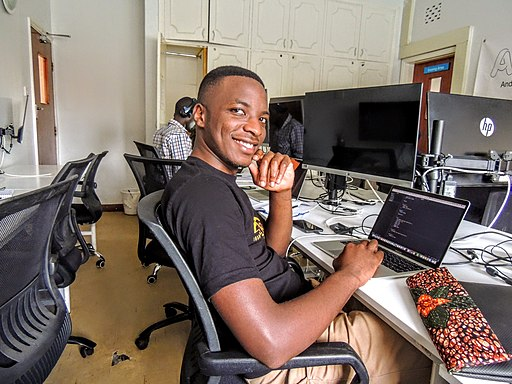
\includegraphics[width=.7\textwidth]{./assets/bob.jpeg}

        \textbf{\Large{...and it continues with Bob}}
    \end{center}
\end{frame}

\begin{frame}
    \begin{center}
        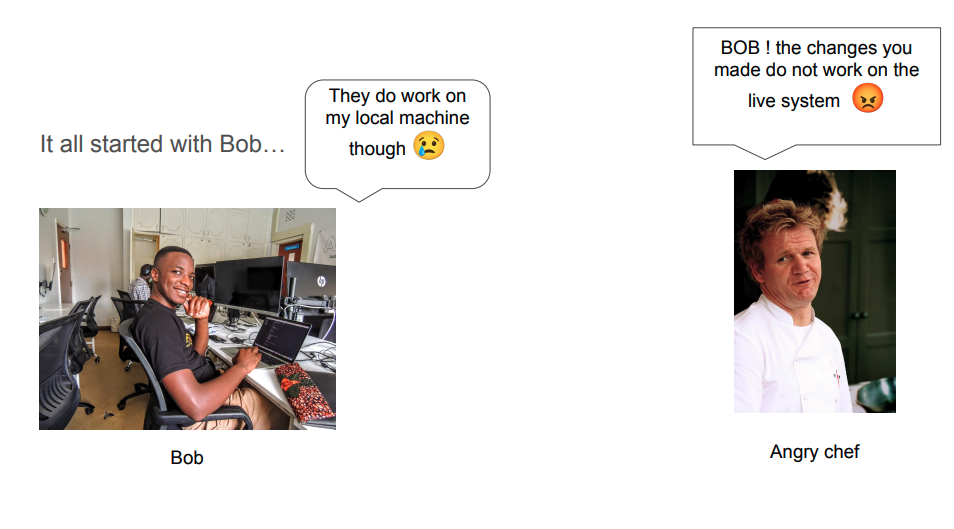
\includegraphics[width=.8\textwidth]{./assets/bob2.png}
    \end{center}
\end{frame}

\begin{frame}{Bob has learnt the lesson...}
    \begin{center}
        
\includegraphics[width=.9\textwidth]{./assets/argocd}
    \end{center}
\end{frame}


\begin{frame}
    \begin{center}
        
\includegraphics[width=.7\textwidth]{./assets/microservice_love.jpeg}
    \end{center}
\end{frame}

\begin{frame}{Extreme examples...}
    \begin{center}
        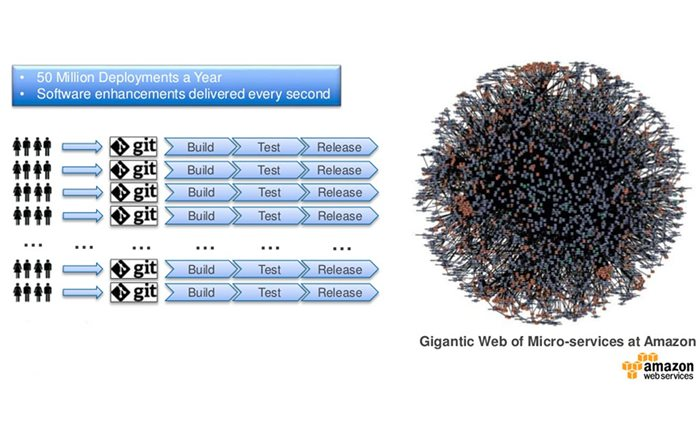
\includegraphics[width=.8\textwidth]{./assets/aws_microservices}
    \end{center}
\end{frame}

\begin{frame}{Everybody loves microservices}
            \begin{itemize}[<+->]
            \item Big promise: Independent deployability
            \item Fast feedback loops
            \item Strong team focus, ideally crossfunctional
            \item Loosely coupled architecture
            \item Fast onboarding
            \item Cost-efficiency on the long run
            \item Cloud native
            \item Tech-agnostic approach
            \item Scalability out of the box
            \item Improved Security (no SPOF, no SPOC)
            \item Optimized Time to Market
            \end{itemize}
\end{frame}

\begin{frame}{Everybody loves microservices}
\begin{columns}
    \begin{column}{0.6\textwidth}
        \begin{shadequote}
            \small{
            \hspace{.5cm} Chief among the benefits of service-enabling an enterprise's
            application landscape are \textbf{increased organizational agility} and
            \textbf{reduced overall cost} of implementing change.

            \vspace{.3cm}

            A SOA increases organizational agility by placing high-value business functions
            in \textbf{discrete, reusable services}, and then connecting and orchestrating
            these services to satisfy core business processes.

            \vspace{.5cm}
            It reduces the cost of change by \textbf{reducing the dependencies} between services,
            allowing them \textbf{to be rapidly recomposed and tuned} in response to change or
            unplanned events.
            }
        \end{shadequote}
    \end{column}
    \begin{column}{0.4\textwidth}
        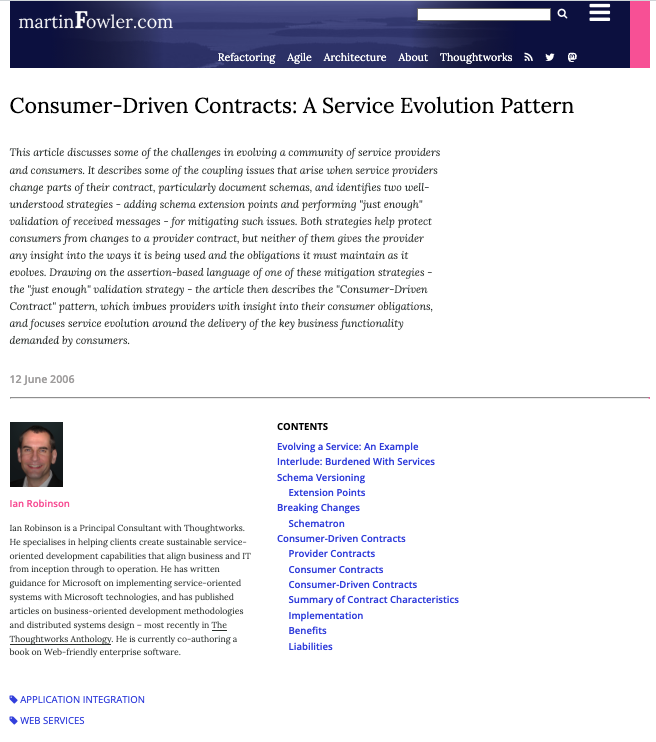
\includegraphics[width=1\textwidth]{./assets/ian_robinson}
    \end{column}
\end{columns}
\end{frame}


\begin{frame}{Is always a tradeoff}
\begin{columns}
    \begin{column}{0.6\textwidth}
        \begin{shadequote}
            \hspace{.5cm}
            There is only one hard rule in software development:
            \textbf{Everything is a tradeoff}.

            \vspace{.3cm}

            -- Neal Ford
        \end{shadequote}
    \end{column}
    \begin{column}{0.4\textwidth}
        
\includegraphics[width=.8\textwidth]{./assets/software_architecture}
    \end{column}
\end{columns}
\end{frame}
